\graphicspath{{experimental-description/}}

\chapter{Summary and Experimental Aims}

In the background section, I laid out a number of general theoretical
orientations: the RTMD theory, the NDI program and multi-system analysis of
cognition. Our findings so far argue strongly for educational opportunities in
the domain of global climate change. In addition, we have been able to engage
individuals with both emotional and more conceptual aspects of psychological
processing in our educational interventions. I have not yet, however, provided
an analysis of NDI style climate interventions, or attempted to use the related
constructs available in the RTMD theory in the construction or enhancement of an
intervention. An NDI intervention has been developed and administered, and
analysis is underway.  Time permitting, the most proximal evolution and perhaps
nationalism constructs will be evaluated for their ability to influence
reasoning or learining about climate.

\begin{table}
\begin{tabular}{p{0.5\textwidth}p{0.5\textwidth}}
Result & Interpretation \\ \hline \hline
Objective scores of participant knowledge increase markedly from pre- to
post-test. & Even in relatively well-educated populations, individuals are
largely ignorant of the mechanism via which greenhouse gases increase global
mean temperature. However, this can be improved with a compact description. \\ \hline
The aggregate of climate change attitudes are improved from pre- to post-test. &
Continuing the above, individuals’ attitudes can also be influenced in a
positive way by a compact explanation. Teaching about the mechanism of global
warming yields shifts in attitudes! \\ \hline
Self-rated knowledge is positively correlated with objectively scored knowledge
when assessed prior to instruction. & Naïve individuals are at least somewhat
correct in their assessment of their knowledge of climate change relative to
their peers’ knowledge. \\ \hline
After instruction, the correlation between self-rated knowledge and objectively
scored knowledge reverses in the “Sandwich” group  & The sandwich intervention
appears to destabilize individuals’ metacognitive assessment of their own
knowledge. The more they learn, the less they think they know! (Note, post-test
correlations in the “No pre-test” group were not-quite-marginally positive.)
Note that the amount known initially is not predictive of self-rated knowledge,
or even objective post-test knowledge. \\ \hline 
Reported surprise is greater when individuals provide an explanation prior to
instruction. & As with results in the NDI paradigm, eliciting a participant’s
“best guess” may reduce post-hoc rationalization, thus increasing feelings of
surprise. This may be critical to obtaining the above-mentioned
“destabilization” of metacognition about one’s knowledge.  \\ \hline
Post-test self-rated knowledge is negatively correlated with surprise ratings in
the “No pre-test” group. & Again, if surprise is taken as a proxy for learning,
we find that such learning may even destabilize metacognition without the
enhancement provided by eliciting a participant’s best guess prior to
instruction.  \\ \hline
Global warming attitude ratings were not (significantly) correlated with
objective knowledge scores. &
It appears that self-assessment of knowledge--which is correlated with global
warming attitude ratings as well as objectively scored knowledge on various
tests--may be a critical link to obtaining attitude change via scientifically
grounded education. \\ \hline
\end{tabular}
\caption{Summary of results from mechanism study}
\label{table:mech-summary}
\end{table}

\begin{table}
\begin{tabular}{p{0.5\textwidth}p{0.5\textwidth}}
Result & Interpretation \\ \hline \hline

Estimation is more likely to improve than worsen after a delay of a day or more.
&
People will learn from a minimal intervention: providing participants with feedback after an estimation.
\\ \hline
Surprise is predictive of improved estimation. &
\multirow{3}{*}{\parbox{0.5\textwidth}{\vskip\baselineskip Surprise and metacognitive 
        assessments of memory may index separable cognitive processes. In
        particular, individuals may gain knowledge (in the form of an improved
        estimation) with no metacognitive awareness that they have done so.}} \\
\cline{1-1}
Metacognitive assessment of memory is predictive of improved estimation. & \\
\cline{1-1}
Surprise and metacognitive assessments of memory may index separable cognitive
processes. In particular, individuals may gain knowledge (in the form of an
improved estimation) with no metacognitive awareness that they have done so. &
\\ \hline
\end{tabular}
\caption{Summary of results from NDI memory study}
\label{table:two-summary}
\end{table}

In chapter~\ref{chap:mechanism}, we observed (for now) isolated probabilistic
dependencies as shown in fig.~\ref{fig:causal-mechanism}, and I have included a more complete
summary of results in table~\ref{table:mech-summary}. Chapter~\ref{chap:two}
found the probabilistic structure expressed in fig.~\ref{fig:causal-two}, and again I
have included a more complete summary in table~\ref{table:two-summary}. Recall
that in the NDI study, we are unable to attribute causality, while in the
mechanism study, due to the nature of the experimental manipulation, we can
assume the relationship between pre-existing knowledge and surprise is sound as
well as the mechanistic knowledge intervention's effect on climate change
acceptance. Below, I will lay out the results that need to be solidified from
the above research, as well as providing a few additional questions to be
answered by the thesis.

As summarized by figures~\ref{fig:causal-mechanism} and \ref{fig:causal-two}, we have
managed to establish some predictive links between measurable variables. There
remain, however, various gaps which can be filled in by relatively obvious
variations on the experiments already done. In addition to the analysis of
existing data, I'm proposing one significant experiment per subsection below. In
addition, below I propose an additional 3 replication experiments using more
general populations. These experiments are intended to elucidate a set of links
such as those shown in fig.~\ref{causal3}.

\begin{figure}
\begin{center}
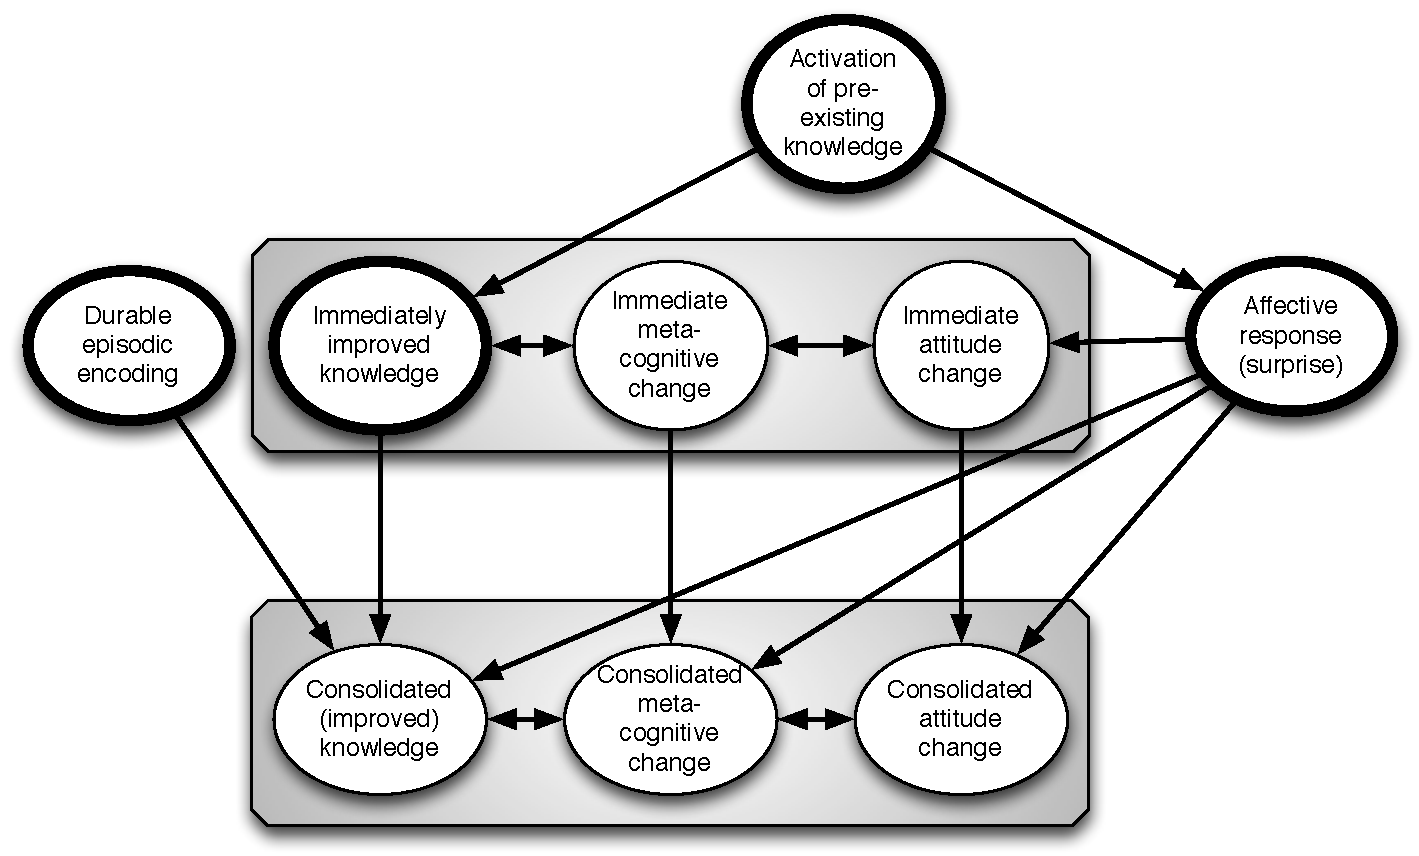
\includegraphics[width=\textwidth]{causal3.pdf}
\end{center}
\caption{A graphical model representing the potential relationships elucidated
    by the proposed experiments. Subjects internal representations are
    surrounded by grey boxes. Points of experimental manipulation are ringed by
    thick lines.}
\label{causal3}
\end{figure}

These experiments will draw on two forms of factual information: a
mechanistic description of the ``greenhouse effect'' and a number of lists of
numerical quantities that pertain to climate change and evolution. For the
purpose of the thesis, these items will be treated separately as opportunities
to elicit psychological processing and subsequent belief and attitude changes.

% In an ideal wold, this would probably get moved to the intro? Do this for
% thesis.
\section{A bit more theory}

One of the more established models of psychological processing of persuasive
messages is the Elaboration Likelihood Model \cite{petty_elaboration_1999}.
This model is (as might be expected) quite Elaborate, but for our current
purpose, it serves to note the following central observation in ELM research.
Specifically, changes in attitudes appear to be driven by at least two modes of
processing (or perhaps a spectrum between these modes) in which new information
may be deeply ``elaborated'' in a central process, or may alternatively be
incorporated peripherally via less effortful processing, such as heuristic or
emotional processing. Of critical concern to our educational goal, effortful
processing tends to yeild shifts that are durable and resistant to subsequent
counter-persuasion. Such persuasion might be crucial to the prevention of social
phenomena such as the gradual erosion of public acceptance of Climate Change
since the spike around the publication of ``An Inconvenient Truth'' 
\cite{leiserowitz_climate_2010}.

Yet another model of belief revision and behavioral change are the Theory of
Reasoned Action and the more elaborated Theory of Planned Behavior
\cite{montano_theory_2008}. In particular, the model posits that sets of
relatively concrete beliefs yeild more general attitudes (expressed as a latent
variable). These attitudes in turn guide individuals' behavior.  Here, I will
use a similar break-down of participants' mental representations, but introduce
an additional level of distinction. These distinctions may not be sharp in all
cases, but for the purposes of this experimental plan, they should be quite
clear. At a basic level, all of the experiments proposed herein operate at the
level of \emph{factual knowledge} (e.g., percentage decrease in ice in a
particular location). This knowledge in turn supports \emph{beliefs} regarding
the veracity of, e.g., anthropogenic climate change. Finally, I will refer to
\emph{attitudes} as consisting of an emotional link to some knowledge or belief.
Criticaly, the target of the emotional link needn't be accepted as true!

A recent model regarding the relationships and learning dynamics between
knowledge and emotional associations is the HOTCO model \cite{thagard_hot_2006}.
In the taxonomy I propose above, facts and beliefs could in principal exist
purely in the domain of ``cold cognition.'' In other words, one could hold ideas
about ice melt and even the reality of climate change solely on the basis of
evidence and inference.  Attitudes (as described above) are inherently emotional
(or ``hot''), however. As described by Thagard, the inferential links between
underlying facts and beliefs and their supported attitudes, such as concern
about climate change, will effect emotional responses to those supporting ideas.
So, for example, a person may have an attidue in which they worry about their
grandchildren's safety and health in the future. If we establish a coherent link
between climate change and this pre-esisting worry, that individual will then
come to worry about climate change. Emotional associations may similarly be
propigated to more basic factual knowledge, such as ice melt in a particular
location.

\section{Intentionally unanswered questions}

Prior to this writing, I have proposed a good number of potential experiments.
Due to pragmatic constraints, only a portion of these will be included in the
proposed thesis. For clarity, I include here a brief list of questions that I
plan to answer with work \emph{subsequent} to the thesis:

\begin{itemize}
    \item To what extent will reasoning and learning about "toy worlds" reflect
        reasoning and learning about real-world scenarioes in which individuals
        have a real, vested interest? Note - this is probably the most common
        question I get when discussing my work, so worth addressing even to get
        the negative result that I anticipate.
    \item What is the relative effectiveness of the various sorts of
        interventions employed here? For example, is suprising numerical
        information more or less effective at eliciting behavioral change than,
        say, appeals from authority or scientific exposition?
    \item To what extent can we characterize the nature of surprise and other
        affective responses at the physiological level? Can we observe emotional
        expressions using video capture? What about measures of respiration,
        heart rate, etc.?
\end{itemize}

\section{Central constructs and Aims}

Primary concern is behavioral change. For the purposes of these studies, we rely
primarily on measures of attitude (including expressed attitudes about planned /
anticipated behavior).

The primary measures are 

\begin{enumerate}
    \item Metacognition about one's knowledge (as it pertains to both the
        specific materials in a given study, as well as potentially the domain
        of climate change in general).
    \item Actual knowledge and change in knowledge (learning).
    \item Affective response to the materials being learned (surprise).
    \item Attitudes regarding climate change.
\end{enumerate}

In addition, a primary manipulation of interest is the elicitation (or not) of a
participant's prior knowledge. This has been shown to modulate surprise in some
of our initial data on climate change, and has been shown to modulate learning
in other studies mentioned above.

% Combine these "aims" with above

\subsection{Aim 1}

\textbf{Attempt to replicate existing effects across both mechanism and NDI based
    educational interventions, obtaining necessary statistical power where
    necessary}

% Determine the (large, obvious) interactions between (potentially)
%     concurrent psychological processes involved in the reading and understanding
%     of factual messages.

\begin{enumerate}
    \item At present, we have only observed reliable shifts in attitudes in UC
        Berkeley undergraduates. We have an existing dataset from UT
        Brownsville, but it is critical to establish the generality of our main
        findings by obtaining a broad sample.
    \item Of central interest from a psychological point of view, we have shown
        (via the mechanism manipulation) that increase in knowledge about
        climate change yeilds shifts in attitudes. However, we were unable to
        obtain a reliable relationship between attitudes and other experimental
        constructs. I expect that with more subjects, between subject
        variability in real and / or self-rated knowledge will significantly
        predict attitude change.
\end{enumerate}

%% This is largely similar to the above

% There are four separable (though not necessarily completely distinct) forms of
% psychological processing that will be measured: 
% 
% \begin{description}
%     \item[Durable episodic encoding] Participants will evaluate the extent of
%         their own learning. Specifically, subjects will be asked to make
%         remember / know style judgements on a numerical scale, as done in
%         experiment one. In addition, episodic encoding may be probed using
%         source detail memory. It should be noted that some degree of episodic
%         encoding is likely engaged for all items, but is simply not retained
%         (i.e., consolidated) in some cases. 
%     \item[Improved knowledge] Participants' actual improvements in their ability
%         to produce specific information. This will be measured either as
%         proximity to a correct numerical answer, or by using a rubric we've
%         developed to evaluate mechanistic descriptions.
%     \item[Interaction with pre-existing knowledge base] Some interaction with
%         participants' pre-existing knowledge is certain to occur. This can
%         manipulated, however, by asking participants to provide their own
%         estimates or explanations before providing them with the correct answer.
%         For the current set of experiments, we will not seek to suppress such
%         interactions.
%     \item[Affective response] Participants will be asked directly to evaluate
%         their reactions to presented items. In addition, for some experiments,
%         participants will be monitored directly using audio, video and
%         psysiological monitoring equipment (currently installed in Tolman 5503).
% \end{description}

\subsection{Aim 2}

\textbf{Extend the scope of data collected, in terms of temporal delay, number
    of participants and depth of survey / interview questions to establish
    further links between established theoretical constructs}

\begin{enumerate}
    \item Evaluate the longitudinal effects of our interventions on both
        knowledge and attitudes. To the extent possible, also probe for changes
        in behavior (or planned behavior).
    \item Refine our understanding of participant attitudes and responses. In
        particular, evaluate the meaning of subject responses on the
        ``surprise'' scale, and refine our assessment of climate change beliefs
        and attitudes.
\end{enumerate}

% Develop a predictive model for the durability and extent of belief and
%     attitude change from differing forms of psychological processing involved in
%     the reading and understanding of factual messages. As compared to aim 1,
%     here we intent to understand how participants generalize beyond the specific
%     information that they are given.}


